\chapter{Deseño e Implementación}

\section{Módulo de Ficheiros}

O módulo de xestión de ficheiros é un do máis importantes e complexos de todo o programa o cal é lóxico tendo en conta que o programa é un editor de ficheiros.

En canto ao deseño, o principal obxetivo é a extensibilidade do mesmo pois, aínda que o programa está centrado na edición de ficheiros PO e son ests os unicos soportados na actualidade, pretendese que o programa sexa capaz de soportar varios tipos de ficheiros nun futuro. Na figura~\ref{fig:dia_class:files} pódese ver o diagrama de clases deste módulo.

\subsection{Implementación Xenérica}
A implementación da clase \lstinline{File} contén propiedeades para conseguir información sobre o nome e path onde está dito ficheiro, ademáis garda estatísticas sobre o número de mensaxes traducidos, sen traducir ou con tradución difusa. Estas estatísticas actualizanse cada vez que se engade ou elimina unha cadea ou cada vez que esta se modifica. Tamén contén un valor booleano que permite saber se o ficheiro foi modificado. Aparte de métodos para engadir e eliminar cadeas, e para conseguir e modificar os metadatos do ficheiro está clase ten un método para gardar o ficheiro e para analizar o ficheiro. O método para gardar~(\lstinline{save}) emprega o patrón \emph{Template Method\footnote{\href{http://gl.wikipedia.org/wiki/Template_Method_\%28patr\%C3\%B3n_de_dese\%C3\%B1o\%29}{Template Method (patrón de deseño)}}} o cal permitenos actualizar o estado do ficheiro a non cambiado.

Un ficheiro contén instancias de mensaxes~(\lstinline{Message}). As mensaxes teñen como propiedades un estado, orixes, e consellos. A API provee métodos para conseguir e modificar tanto as cadeas orixinais como as traducións na súa forma en singular ou nalgunha das formas plurais. A implementación do método para modificar unha tradución tamén emprega o patrón Template Method para actualizar o estado da mensaxe. Esta clase tamén ten métodos para engadir e eliminar consellos e para obter o contexto da mensaxe.

\begin{figure}[h!]
    \centering
    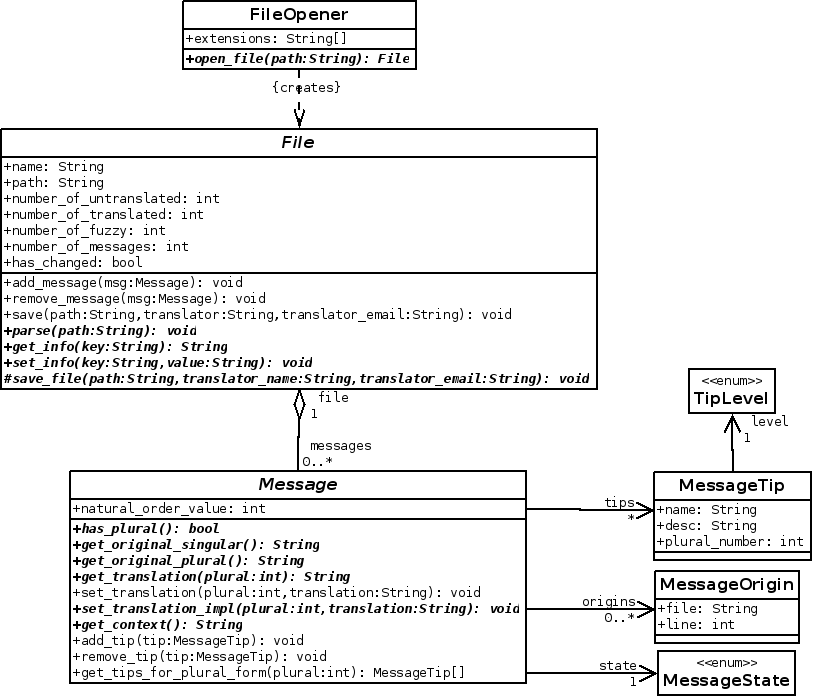
\includegraphics[width=\textwidth]{img/genericfile.png}
    \caption{Diagrama de Clases do módulo ficheiros}
    \label{fig:dia_class:files}
\end{figure}

Ademais a clase \lstinline{FileOpener} recolle un método para crear ficheiros e un conxunto de extensións que se poden abrir con este FileOpener.

\subsubsection{Consellos (Tips)}
Os consellos son a solución que damos para aportar información ao usuario sobre a tradución que está a realizar. Algunha das cousas que pode axudar a indicar esta característica é se a tradución está a ser demasiado longa, se hai algunha palabra que está mal escrita na tradución ou se non emprega a terminoloxía adecuada.

Cada consello ten un nome que debe ser xenerico a cada clase de consello, unha descripción que ten que explicar o problema con detalle, un nivel que indica a gravidade do consello e unha referencia a forma plural a que corresponde dito consello. Ademáis pode conter un ou máis referencias a localización exacta do problema que permitirá destacala na interface gráfica.

A creación de consellos faráse ao modificarse unha cadea e farase a través de plugins.

\subsubsection{Pistas (Hints)}
As pistas amosaranlle ao usuario posibles traducións ou aproximacións as traducións. Estas pistas poden ser obtidas de memorias de traducións, de traducións do mesmo ficheiro noutra linguaxe, ou da tradución directa por exemplo.

Cada instancia dunha pista~(\lstinline{Hint}) contén a tradución suxerida, unha cadea que identifica a orixe de dita pista e un valor que indica a precisión de dita suxerencia.

De igual forma que no caso dos consellos a creación de pistas correrá ao cargo de plugins creados a tal proposito. Neste caso actualizaranse as pistas de cada mensaxe ao selecionalo mesmo na interface.

\subsection{Ficheiro PO}
A implementación especifica para ficheiros PO extende as clases \lstinline{File}, \lstinline{FileOpener} e \lstinline{Message} abstractas para implementar os metodos e permitir empregar ficheiros PO.

Para a analise e a actualización dos ficheiros PO empregaremos a biblioteca gettext-po. No momento no que se iniciou a implementación deste módulo non existía implementación destal librería en Vala polo que tivemos que crear uns \emph{bindings} para poder empregala.

Tanto a clase PoFile como a clase PoMessage delegan a maior parte dos seus métodos nas instancias das clases dos bindings da biblioteca GettextPo File e Message respectivamente. Desta forma faise un claro uso do patrón \emph{Adapter\footnote{\href{http://gl.wikipedia.org/wiki/Adapter_\%28patr\%C3\%B3n_de_dese\%C3\%B1o\%29}{Adapter (patrón de deseño)}}}.

\begin{figure}[h!]
    \centering
    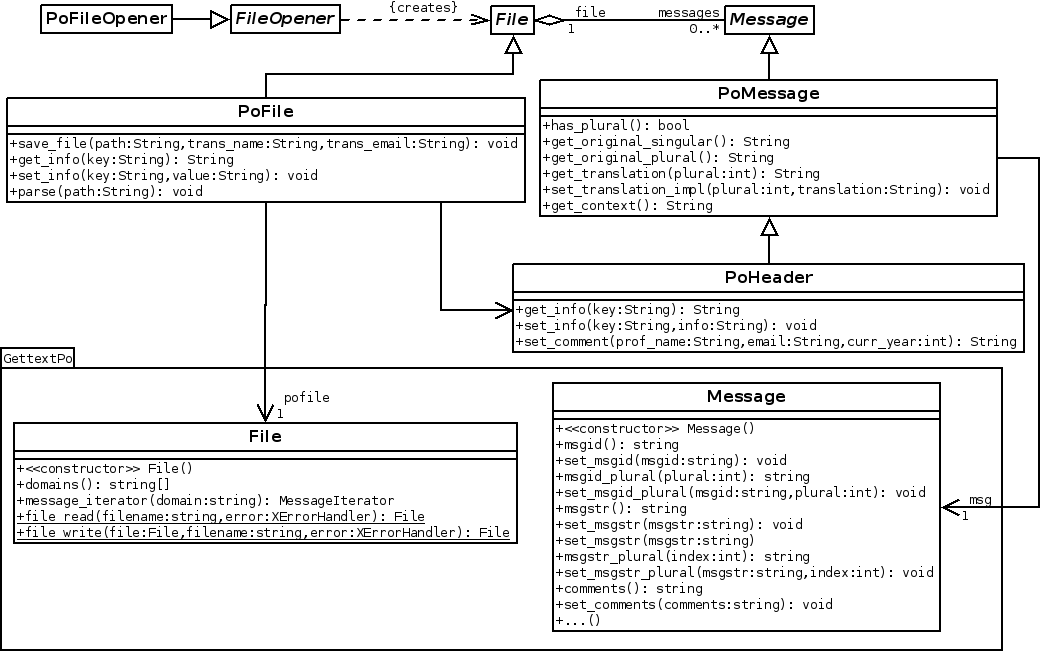
\includegraphics[width=\textwidth]{img/pofile.png}
    \caption{Diagrama de Clases do ficheiro PO}
    \label{fig:dia_class:pofile}
\end{figure}

De forma adicional a clase PoFile contén unha instancia da clase PoHeader esta clase que extende e PoMessage correspondese aos metadatos que se atopan nos ficheiros PO na tradución da cadea baleira. É ten meodos para obter e modificar metadatos e para actualizar os datos dos autores das traducións de dito ficheiro. A clase PoFile delega nesta clase a hora de conseguir e modificar metadatos e tamén cando garda un ficheiro.

A clase \lstinline{PoFileOpener} so é capaz de abrir ficheiros con extensión PO e simplemente emprega o método parse da clase ficheiro para crear unha nova instancia.

\subsubsection{Implementación dos bindings}
Como xa mencionamos vimonos na obriga de crear nós os bindings para a biblioteca gettext-po. Vala é unha linguaxe deseñada para permitir o acceso a outras bibliotecas escritas en C, especialmente se se trata de bibliotecas baseadas en GObject. Despois de todo Vala emprega C como linguaxe intermedio. A biblioteca gettextpo non é unha biblioteca baseada en GObject polo que a creación destes bindings é un pouco máis complicado.

Para poder empregar unha biblioteca escrita en C no noso programa escrito en Vala so temos que crear un ficheiro con extensión VAPI que conteña en sintaxe Vala as clases da biblioteca engadindo unhas etiquetas que permitan a súa tradución ao código C correcto. No Fragmento de código~\ref{lst:bindingsgettext} podemos ver parte dos bindings creados para a biblioteca gettextpo.

\lstset{language=[sharp]C}
\begin{lstlisting}[label=lst:bindingsgettext,caption=Bindings da biblioteca GettextPo]
[CCode (cprefix = "Po", lower_case_cprefix = "po_")]
namespace GettextPo {

    [CCode(cheader_filename = "gettext-po.h", cname="struct po_file", free_function="po_file_free")]
    [Compact]
    public class File {

        [CCode (CCode = "po_file_create")]
        public File();

        [CCode (array_length = false, array_null_terminated = true, cname="po_file_domains")]
        public unowned string[] domains ();

        [CCode (cname="po_file_write")]
        public static unowned GettextPo.File file_write (GettextPo.File file,
                            string filename,
                            XErrorHandler handler);
        [...]
    }

    [CCode(cheader_filename = "gettext-po.h", cname="struct po_message")]
    [Compact]
    public class Message  {

        [CCode (cname="po_message_create")]
        public Message();
        public unowned string msgid ();
        public unowned string? msgid_plural ();
        [...]
\end{lstlisting}

Como podemos ver o traballo prácticamente limitase a establecer o parametro \lstinline{cname} en cada clase e método. Hai que ter en conta que non sempre e necesario especificar este parámetro pois as bibliotecas empregan case sempre unhas normas de nombrado que fan que usen primeiro o nome da biblioteca, despois o nome da clase e logo o nome do método separado por barras baixas. Desta forma no método da biblioteca \lstinline{po_message_msgid()}, \emph{po\_} corresponde o nome da biblioteca, \emph{message\_} ao nome da clase e \emph{msgid} ao nome do método. Os bingings de vala empregan estas normas para nomear os métodos polo que en ocasións non é necesario especificar o parametro cname. Isto sucede, como se pode ver no fragmenteo de código anterior no caso da clase Mensaxe (\lstinline{Message}).

Ademais e necesario especificar o nome do ficheiro cabeceira que se emprega e no caso de que o tipo de retorno sexa un array temos que especificar máis parametros como acontece no método \lstinline{domains()} da clase File. Por último é importa especificar a pertenza de cada valor e os métodos correctos para liberar as instancias desta forma evitaremos que haxa perdas de memoria e fallos de segmentación.

\section{Módulo de Linguaxes}
O módulo de linguaxes xestiona os linguaxes e formas plurais existentes. Contén dúas clases, a clase \lstinline{Language} e a clase \lstinline{PluralForm}. Estas dúas clasen proveen un método estático para obter as instancias existentes. Estas instancias creanse a primeira vez que se carga a clase consultando unhas bases de datos que consisten nuns ficheiros JSON\footnote{\href{http://gl.wikipedia.org/wiki/JSON}{JSON}}.

A cada instancia dunha linguaxe contén o nome da linguaxe, o seu código empregando a norma ISO 639-1 a súa forma plural e o email do equipo de tradución por defecto. Engadimos o idioma do equipo de tradución por defecto para autocompletar este campo no perfil do usuario. No Fragmento de Código~\ref{lst:languages} podemos ver un fragmento do ficheiro JSON contendo as linguaxes.

\begin{lstlisting}[label=lst:languages,caption=Fragmento da Base de Datos de Linguaxes]
  {
    "languages" : [
      [...]
      {
        "code" : "sl",
        "name" : "Slovenian",
        "pluralform" : "nplurals=4; plural=(n\%100==1 ? 1 : n\%100==2 ? 2 : n\%100==3 or n\%100==4 ? 3 : 0);",
        "default-team-email": ""
      },
      {
        "code" : "so",
        "name" : "Somali",
        "pluralform" : "",
        "default-team-email": ""
      },
      {
        "code" : "es",
        "name" : "Spanish; Castilian",
        "pluralform" : "nplurals=2; plural=(n != 1);",
        "default-team-email": "gnome-es-list@gnome.org"
      },
      [...]
    ]
  }
\end{lstlisting}

En canto a clase \lstinline{PluralForm}, esta clase inclue o número de plurais, a expresión desa forma plural e un conxunto de tags. Estos tags pretenden faculitar ao usuario a identificación de que número corresponde a cada forma plural. No Fragmento de Código~\ref{lst:plurals} pódemos ver unha parte da base de datos de formas plurais.

\begin{lstlisting}[label=lst:plurals,caption=Fragmento da Base de Datos de Plurais]
  {
    "forms" : [
      {
        "expression" : "nplurals=2; plural=(n > 1);",
        "number_of_plurals" : 2,
        "tags" : [
	  {
            "number" : 0,
            "tag" : "Equal to 0 or 1"
	  },
	  {
            "number" : 1,
            "tag" : "Greater than 1"
	  }
	]
      },
      [...]
    ]
  }
\end{lstlisting}

\section{Interface Gráfica}
A interface gráfica é unha das partes a que máis tempo lle dedicamos neste proxecto. O obxetivo dende o principio foi construir algo simple pero potente que permitira ao usuario editar os ficheiros PO de forma sinxela pero que aportase fose capaz de aportarlle moita información que lle axudase a facer a tradución.

\subsection{Evolución}
Durante a execución do proxecto probamos diferentes formas da interface gráfica ata chegar ao resultado actual. Estas versións pretenden imitar programas existenttes e obedecen xeralmente a conversacións con traductores.

\subsubsection{Primeira Versión: moi semellante a GTranslator}
Para comezar a traballar e tras amosar varios mockups nos reportes recibindo feedback sobre eles decidimos facer unha interface de usuario moi parecida a de GTranslator. Esta interface inclue bloques para a lista de mensaxes, editar ditos mensaxes e amosar o contexto. Estos bloques podense mover por toda a interface e incluso separar da mesma xa que estamos empregando a biblioteca GNOME Docking Library. Na Figura~\ref{fig:ui:v1:general} podemos ver o aspecto desta primeira versión da interface.

\begin{figure}[h!]
  \centering
    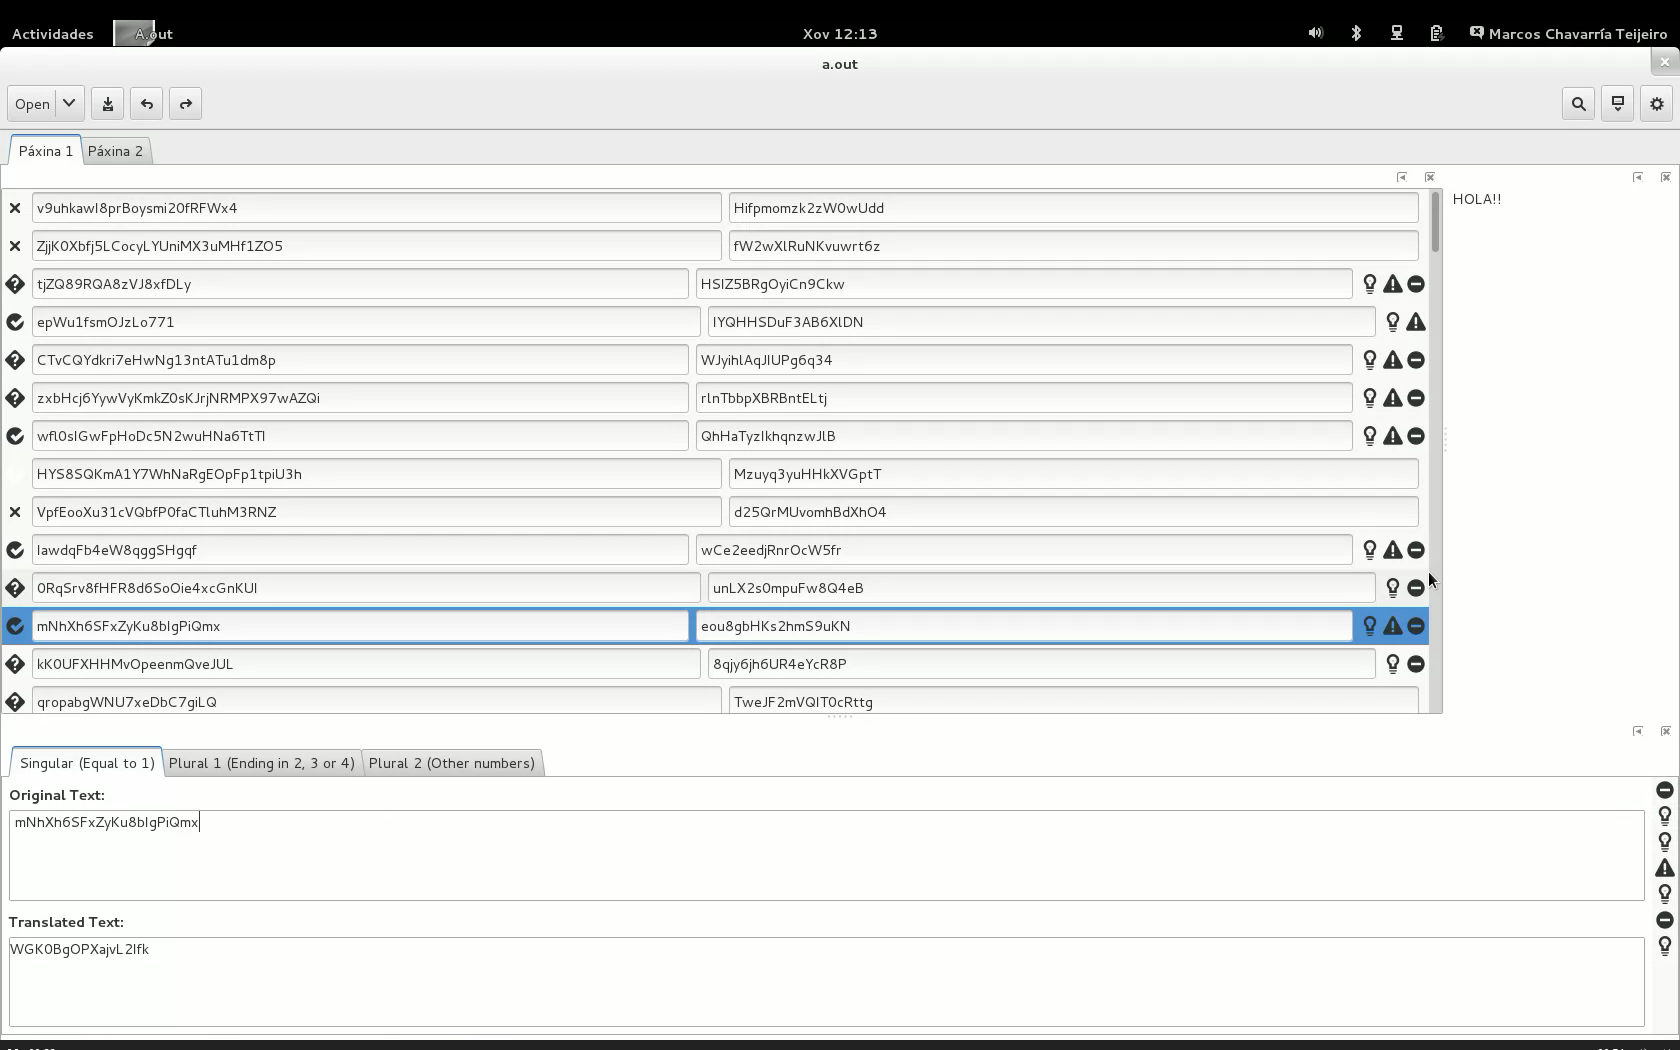
\includegraphics[width=\textwidth]{img/gsoc1_it2_ui.png}
    \caption{Diagrama de Clases do módulo ficheiros}
    \label{fig:ui:v1:general}
\end{figure}

Como podemos ver a interface contén un barra de ferramentas que permite abrir ficheiros, gardalos, desfacer e refacer cambios, buscar no documento e ver as preferencias. Permite abrir diversos ficheiros en varias lapelas. En cada unha das lapelas podemos ver a lista de mensaxes e o widget de edición.

En cada mensaxe da lista, aparte das cadeas orixinal e traducida, podemos ver o estado da cadea e se está ten consellos (Tips) activos e de que nivel de estos. Por outro lado, no widget de edición podemos ver unha lapela por cada forma plural que podemos editar e unha lista vertical con iconos cos consellos. Ao pasar o rato polo consello veremos a súa descripción.

\begin{figure}[h!]
  \centering
  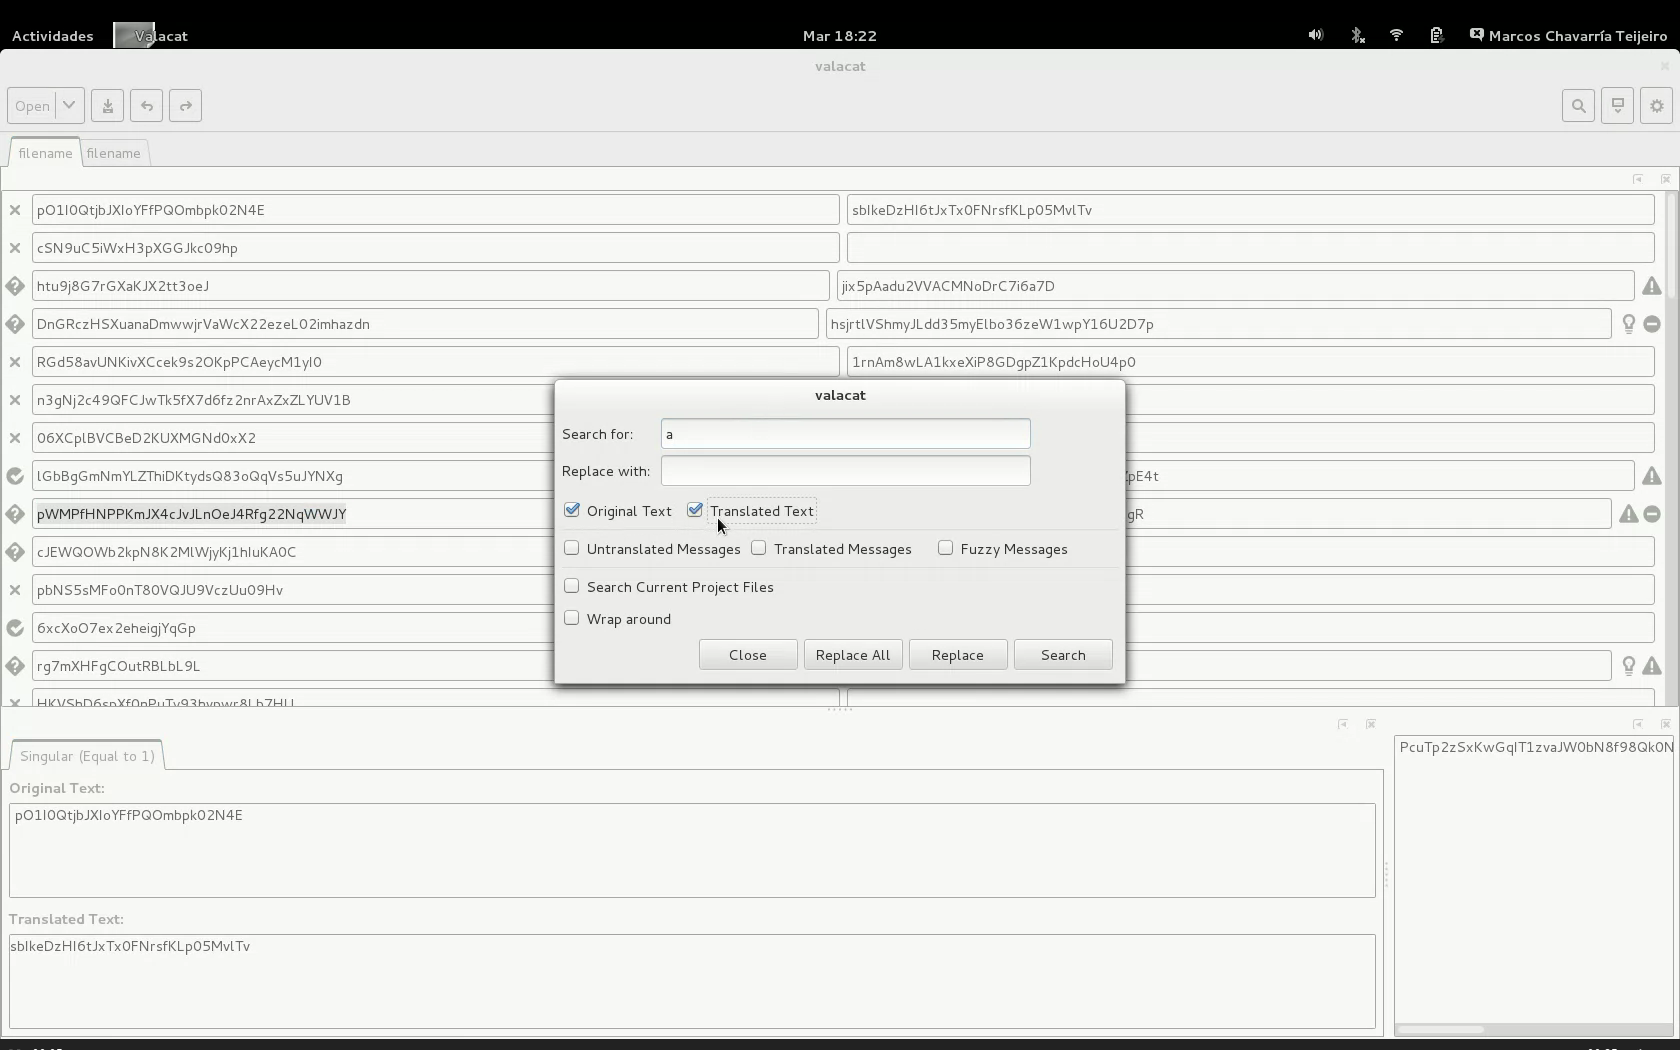
\includegraphics[width=0.4\textwidth]{img/gsoc1_it3_ui.png}
  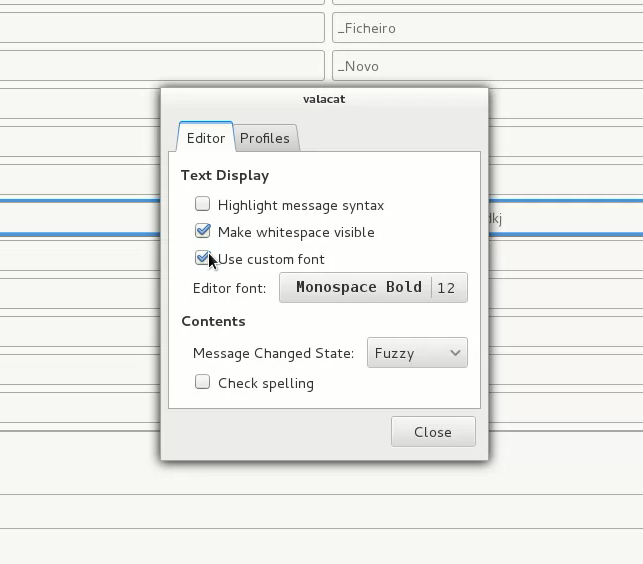
\includegraphics[width=0.4\textwidth]{img/gsoc1_it5_prefs.png}
  \caption{Diagrama de Clases do módulo ficheiros}
  \label{fig:ui:v1:dialogs}
\end{figure}

Como podemos ver na Figura~\ref{fig:ui:v1:dialogs} tanto a hora de xerar unha búsqueda como para ver as preferencias esta interface empregara uns dialogos non modales.

En conversacións en IRC con traductores e anteriores mantenedores de GTranslator chegamos a conclusión de que o uso de GNOME Docking Library era unha mala idea pois significaba un erro de deseño xa que se o usuario tiña que modificaar o apecto da interface é que o deseño non era correcto. Esta biblioteca ademais ten bastantes fallos polo que non era recomendable usala.

Ademais durante a GUADEC, comentaronos da existencia dun widget moito mellor para xestionar a buscas consistente nunha barra horizontal que se desplegaba cando a busca estaba activa.

Por outro lado o resultado desta modelo de interface tampouco era demasiado satisfactorio polo que intentamos probar con unha versión máis cercana ao programa Virtaal.

\subsubsection{Segunda Versión: semellante a Virtaal}
\subsubsection{Terceira Versión}

\subsection{Paneis}

\begin{figure}[h!]
  \centering
    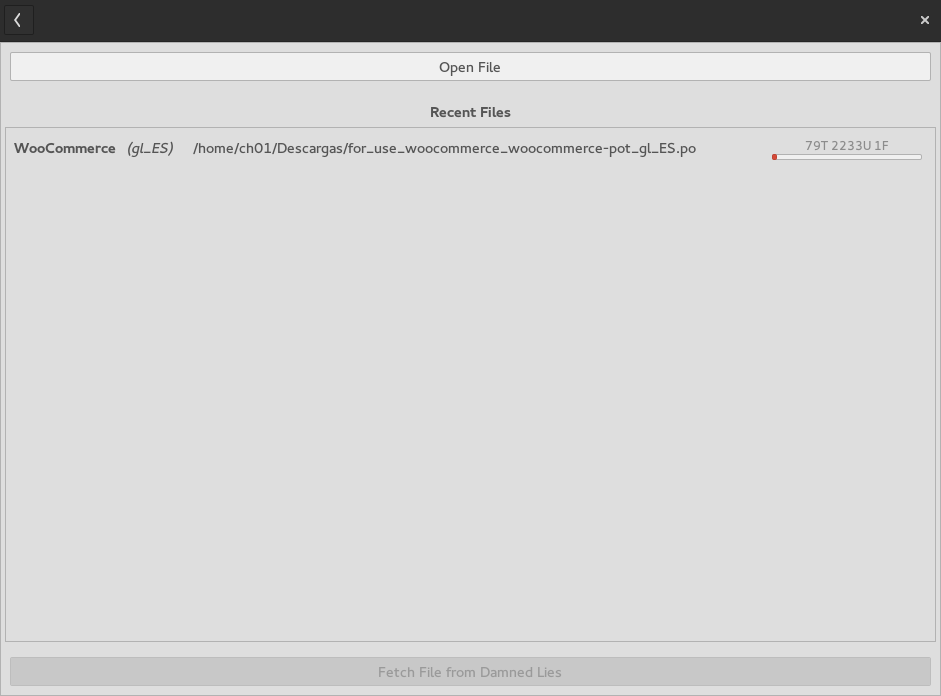
\includegraphics[width=0.8\textwidth]{img/panel_abrir_ficheiro.png}
    \caption{Diagrama de Clases do módulo ficheiros}
    \label{fig:dia_class:files}
\end{figure}

\begin{figure}[h!]
    \centering
    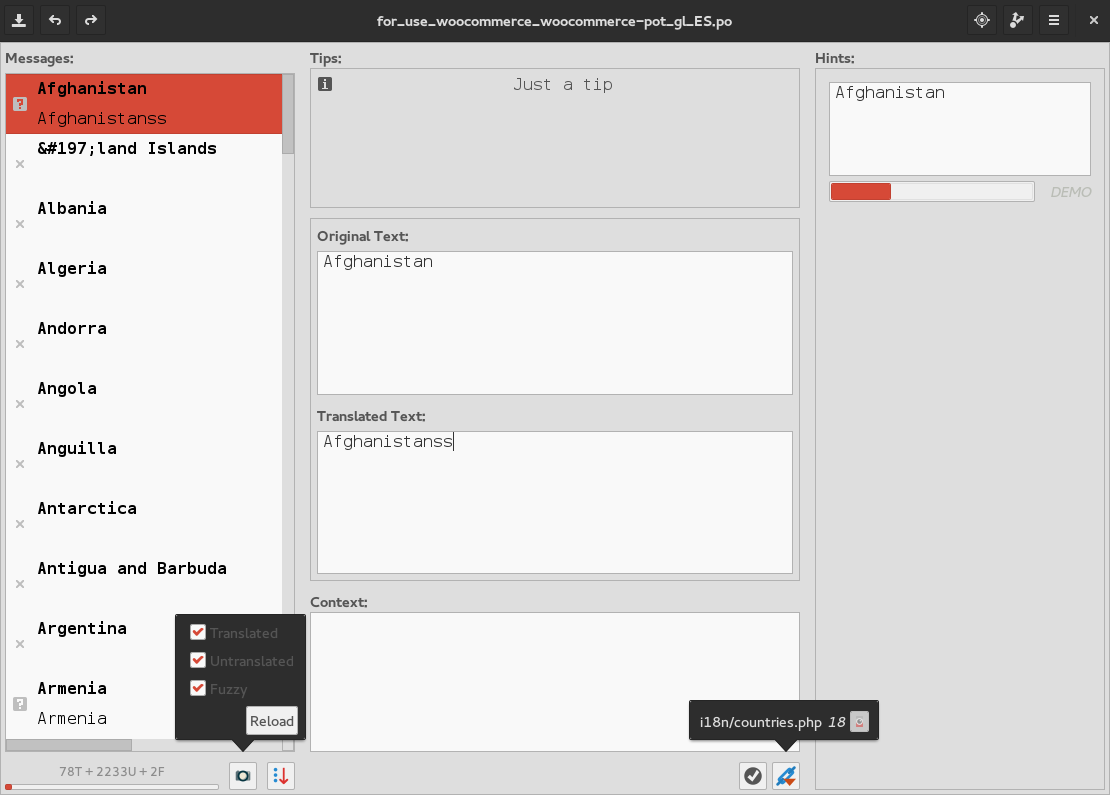
\includegraphics[width=0.8\textwidth]{img/panel_edicion.png}
    \caption{Diagrama de Clases do módulo ficheiros}
    \label{fig:dia_class:files}
\end{figure}

\begin{figure}[h!]
    \centering
    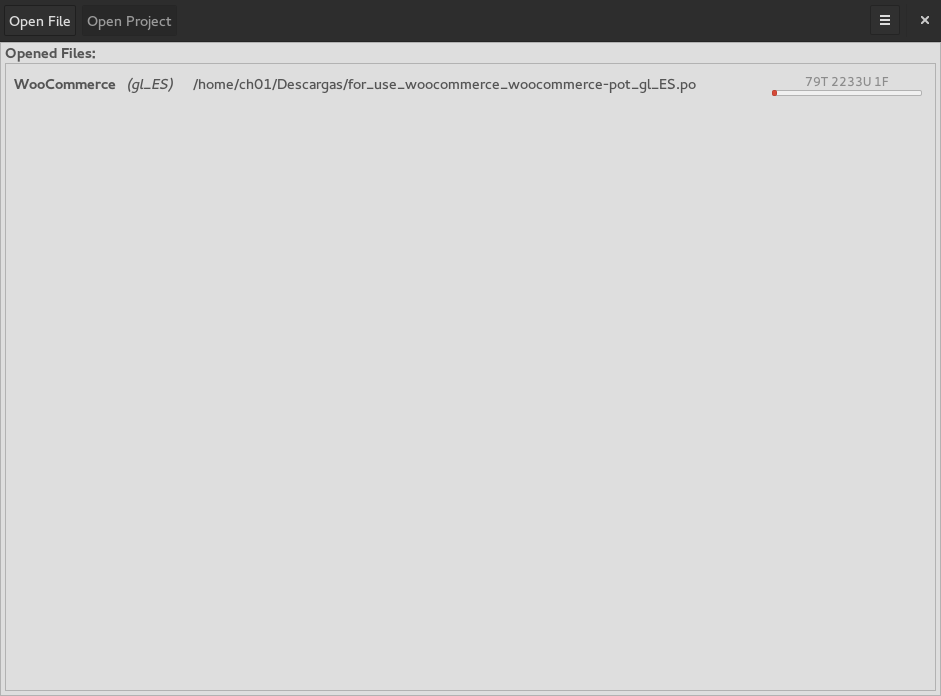
\includegraphics[width=0.8\textwidth]{img/panel_ficheiros_abertos.png}
    \caption{Diagrama de Clases do módulo ficheiros}
    \label{fig:dia_class:files}
\end{figure}

\begin{figure}[h!]
    \centering
    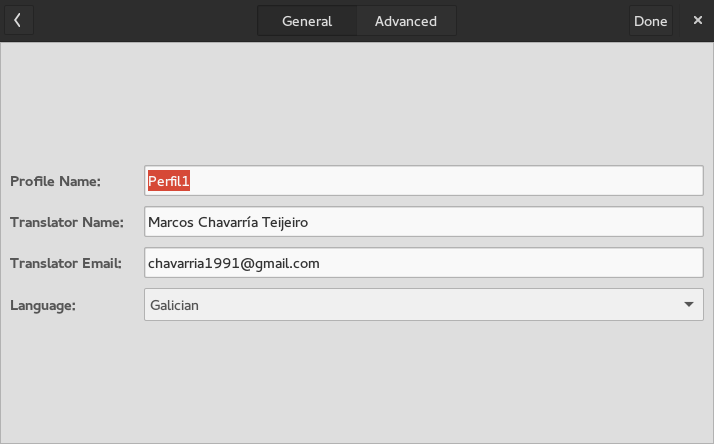
\includegraphics[width=0.8\textwidth]{img/panel_pefil_xeral.png}
    \caption{Diagrama de Clases do módulo ficheiros}
    \label{fig:dia_class:files}
\end{figure}

\begin{figure}[h!]
    \centering
    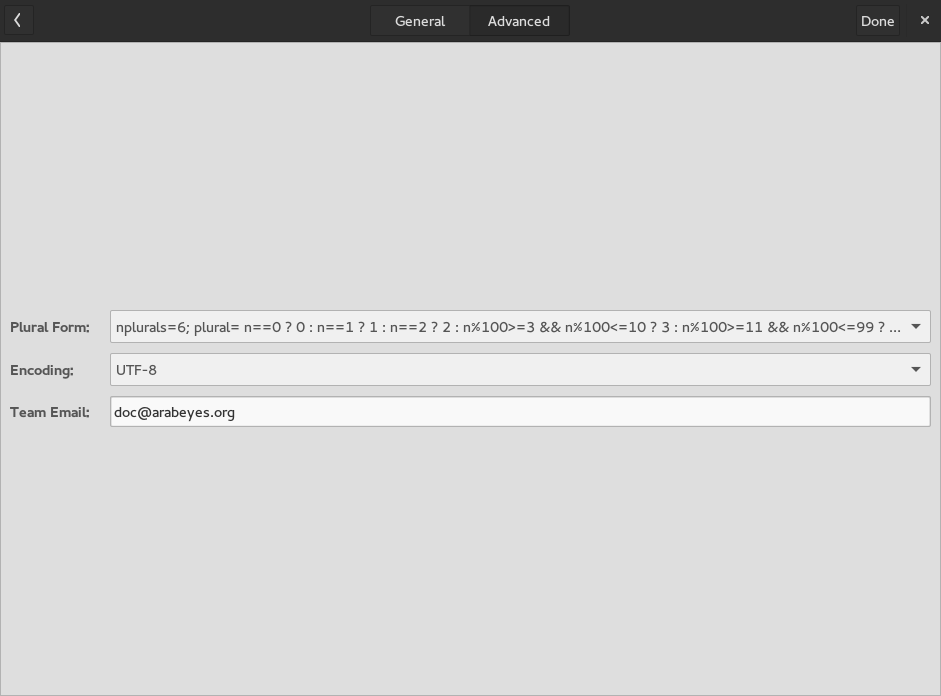
\includegraphics[width=0.8\textwidth]{img/panel_perfil_avanzado.png}
    \caption{Diagrama de Clases do módulo ficheiros}
    \label{fig:dia_class:files}
\end{figure}

\begin{figure}[h!]
    \centering
    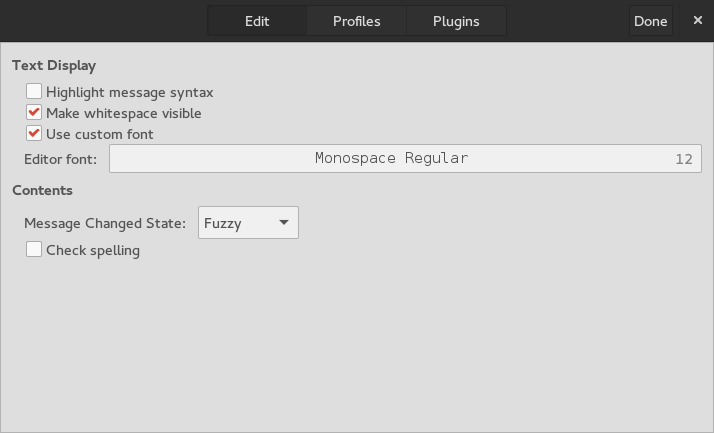
\includegraphics[width=0.8\textwidth]{img/panel_preferencias_edicion.png}
    \caption{Diagrama de Clases do módulo ficheiros}
    \label{fig:dia_class:files}
\end{figure}

\begin{figure}[h!]
    \centering
    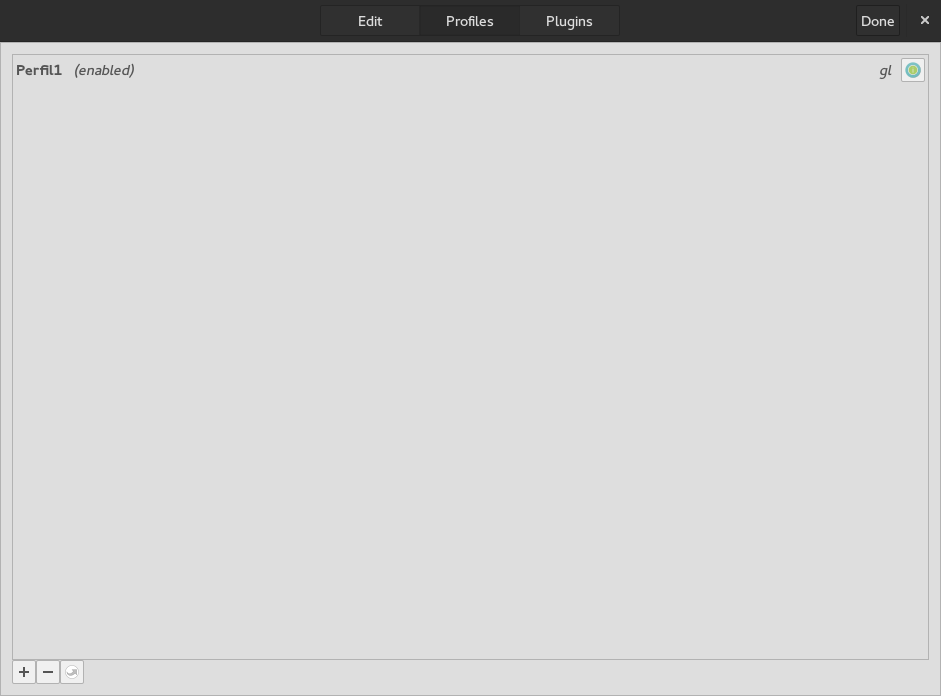
\includegraphics[width=0.8\textwidth]{img/panel_preferencias_perfiles.png}
    \caption{Diagrama de Clases do módulo ficheiros}
    \label{fig:dia_class:files}
\end{figure}

\begin{figure}[h!]
    \centering
    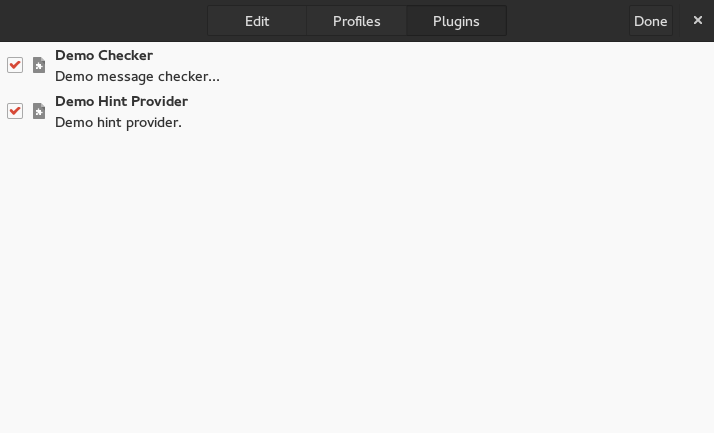
\includegraphics[width=0.8\textwidth]{img/panel_preferencias_plugins.png}
    \caption{Diagrama de Clases do módulo ficheiros}
    \label{fig:dia_class:files}
\end{figure}


\section{Navegación e Busca a través do documento}

\section{Preferencias}

\subsection{Módulo de Perfiles}

\section{Plugins}
